%%%%%%%%%%%%%%%%%%%%%%%%%%%%%%%%%%%%%%%%%
% baposter Landscape Poster
% LaTeX Template
% Version 1.0 (11/06/13)
%
% baposter Class Created by:
% Brian Amberg (baposter@brian-amberg.de)
%
% This template has been downloaded from:
% http://www.LaTeXTemplates.com
%
% License:
% CC BY-NC-SA 3.0 (http://creativecommons.org/licenses/by-nc-sa/3.0/)
%
%%%%%%%%%%%%%%%%%%%%%%%%%%%%%%%%%%%%%%%%%

%----------------------------------------------------------------------------------------
%	PACKAGES AND OTHER DOCUMENT CONFIGURATIONS
%----------------------------------------------------------------------------------------

\documentclass[portrait,a0paper,fontscale=0.285]{baposter} % Adjust the font scale/size here

\frenchspacing

\usepackage{braket}     %required for quantum
\usepackage{mathtools}  %required for quantum
 
\usepackage{graphicx} % Required for including images
\graphicspath{{figures/}} % Directory in which figures are stored

\usepackage{amsmath} % For typesetting math
\usepackage{amssymb} % Adds new symbols to be used in math mode

\usepackage{booktabs} % Top and bottom rules for tables
\usepackage{enumitem} % Used to reduce itemize/enumerate spacing
\usepackage{palatino} % Use the Palatino font
\usepackage[font=small,labelfont=bf]{caption} % Required for specifying captions to tables and figures

\usepackage{multicol} % Required for multiple columns
\setlength{\columnsep}{1.5em} % Slightly increase the space between columns
\setlength{\columnseprule}{0mm} % No horizontal rule between columns

\usepackage{tikz} % Required for flow chart
\usetikzlibrary{shapes,arrows} % Tikz libraries required for the flow chart in the template

\usepackage{epstopdf}

\newcommand{\compresslist}{ % Define a command to reduce spacing within itemize/enumerate environments, this is used right after \begin{itemize} or \begin{enumerate}
\setlength{\itemsep}{1pt}
\setlength{\parskip}{0pt}
\setlength{\parsep}{0pt}
}

\definecolor{lightblue}{rgb}{0.145,0.6666,1} % Defines the color used for content box headers

\definecolor{ourred}{rgb}{0.9,0.0,0.0}

\begin{document}

\begin{poster}
{
headerborder=closed, % Adds a border around the header of content boxes
colspacing=1em, % Column spacing
bgColorOne=white, % Background color for the gradient on the left side of the poster
bgColorTwo=white, % Background color for the gradient on the right side of the poster
borderColor=lightblue, % Border color
headerColorOne=black, % Background color for the header in the content boxes (left side)
headerColorTwo=lightblue, % Background color for the header in the content boxes (right side)
headerFontColor=white, % Text color for the header text in the content boxes
boxColorOne=white, % Background color of the content boxes
textborder=roundedleft, % Format of the border around content boxes, can be: none, bars, coils, triangles, rectangle, rounded, roundedsmall, roundedright or faded
eyecatcher=true, % Set to false for ignoring the left logo in the title and move the title left
headerheight=0.1\textheight, % Height of the header
headershape=roundedright, % Specify the rounded corner in the content box headers, can be: rectangle, small-rounded, roundedright, roundedleft or rounded
headerfont=\Large\bf\textsc, % Large, bold and sans serif font in the headers of content boxes
%textfont={\setlength{\parindent}{1.5em}}, % Uncomment for paragraph indentation
linewidth=2pt % Width of the border lines around content boxes
}
%----------------------------------------------------------------------------------------
%	TITLE SECTION 
%----------------------------------------------------------------------------------------
%
{
\includegraphics[height=8.6em]{leidenland.pdf}} % First university/lab logo on the left
{\bf\textsc{\textcolor{ourred}{The effects of noise on quantum algorithms solving 3-SAT}}\vspace{-0.1em}} % Poster title
{\textsc{\begin{large}Martijn Swenne\end{large} \begin{small}(supervized by Vedran Dunjko)\end{small}\\ \begin{small}Leiden Institute of Advanced Computer Science\end{small}\\[0.5mm]}\begin{footnotesize}\texttt{s1923889@liacs.leidenuniv.nl}\end{footnotesize}} % Author names and institution

%----------------------------------------------------------------------------------------
%	OVERVIEW
%----------------------------------------------------------------------------------------

\headerbox{1. Overview}{name=overview,column=0,row=0}{

\textcolor{ourred}{\textsc{Quantum}} is a term you hear a lot lately. Quantum computing uses quantum-mechanical phenomena, such as superposition and entanglement. A quantum computer is therefor completely different than a classical computer. Whereas a classical computer uses binary digits, which are always in one of two definite states (0 or 1), a quantum computer uses quantum bits, or \textcolor{ourred}{\textsc{qubits}}. These qubits can be in a quantum superposition of states. Quantum computers are extremely powerful, but also very noisy. This is currently a big problem in quantum computers. Quantum computers can speed up certain combinatorial optimization problems, and here I investigate how noise affects the solving of 3SAT problems in particular.

}

%----------------------------------------------------------------------------------------
%	Basics
%----------------------------------------------------------------------------------------

\headerbox{2. Basics}{name=basics,column=0,below=overview}{ % This block's bottom aligns with the bottom of the conclusion block

A \textcolor{ourred}{\textsc{quantum computer}} operates on a register of $n$ qubits using quantum gates and measurement. These $n$ qubits be in any quantum superposition. Quantum states are represented by vectors of a $2^{n}$ dimensional vector space called the Hilbert space. Quantum gates are represented by unitary matrices acting on the state vectors, thereby changing them. Quantum computing elements are typically denoted using the \textcolor{ourred}{\textsc{Dirac}} notation, for instance, the basis state of a single qubit is called ket $\ket{0}$. Qubits and quantum gates can be described with matrices. For instance:

\begin{center}
\vspace{-0.6em}
$\ket{0} = 
\begin{bsmallmatrix}
	1 \\
	0 \\
\end{bsmallmatrix}$
and 
$\ket{1} = 
\begin{bsmallmatrix}
	0 \\
	1 \\
\end{bsmallmatrix}$
\vspace{-0.6em}
\end{center}

Just as in classical computations, where you work with classical logic gates, quantum computations work with quantum logic gates, which are 1 or 2 qubit gates. Unlike classical logic gates, these gates are reversible. For instance, a basic quantum logic gate is the Hadamard gate:

\begin{center}
		$H\ket{0} = \frac{1}{\sqrt{2}}
		\begin{bsmallmatrix}
			1 & 1 \\
			1 & $-$1 \\
		\end{bsmallmatrix}
		\begin{bsmallmatrix}
			1 \\
			0 \\
		\end{bsmallmatrix}
		=	\frac{1}{\sqrt{2}}
		\begin{bsmallmatrix}
			1 \\
			1 \\
		\end{bsmallmatrix}
		=
		\frac{\ket{0}+\ket{1}}{\sqrt{2}}$	
	
		$H\ket{1} = \frac{1}{\sqrt{2}}
		\begin{bsmallmatrix}
			1 & 1 \\
			1 & $-$1 \\
		\end{bsmallmatrix}
		\begin{bsmallmatrix}
			0 \\
			1 \\
		\end{bsmallmatrix}
		=	\frac{1}{\sqrt{2}}
		\begin{bsmallmatrix}
			1 \\
			$-$1 \\
		\end{bsmallmatrix}
		=
		\frac{\ket{0}-\ket{1}}{\sqrt{2}}$
\end{center}

The Hadamard gate puts the qubit in a superposition of basis states. The probability of the resulting qubit being measured in the state is $\ket{0}$ is $(\frac{1}{\sqrt{2}})^{2}=0.5$ as given by the born rule. 

There is another basic quantum gate, which is called the CNOT-gate. This is a controlled-NOT gate. The gate flips the state of the target qubit if and only if the control qubit is $1$.

\begin{center}
\vspace{-1em}
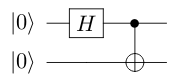
\includegraphics[scale=0.7]{H_CNOT_circuit.png}
\vspace{-1em}
\end{center}

If you now apply a Hadamard gate on the control qubit before a CNOT-gate, the two qubits become \textcolor{ourred}{\textsc{entangled}}. This means that you cannot describe a qubit independently of the state of the other qubit.

Entanglement is a type of quantum correlation, which is at the basis of most of quantum information, and cannot be explained just by classical correlations.
}

%----------------------------------------------------------------------------------------
%	Solving 3SAT
%----------------------------------------------------------------------------------------

\headerbox{4. Solving 3-SAT}{name=solvingSAT,column=2,row=0}{

The \textcolor{ourred}{\textsc{boolean satisfiability}} problem determines if there is a satisfying assignment to a given Boolean formula. A special case of boolean satisfiability is the \textcolor{ourred}{\textsc{3-SAT}}. This means the boolean formula is in CNF where each clause is limited to at most $3$ literals. Such a boolean formula can be written like:

\vspace{-0.5em}
\begin{center}
$F(x_{1}\dots x_{n}) = (l_{1} \lor l_{3} \lor l_{4}) \land \dots \land (l_{1} \lor l_{7} \lor l_{n})$

with $l_{i} = x_{i}$ or $l_{i} = \neg x_{i}$
\end{center}
\vspace{-0.5em}

SAT is proven to be NP-complete. This means that it is not solvable in polynomial time. Quantum computers are also not believed to be able to solve it in polynomial time. However, the \textcolor{ourred}{\textsc{Grover's search}} algorithm can solve it brute force in $O(2^{n/2})$, while a classical brute force solves it in $O(2^{n})$.

\vspace{-0.5em}
\begin{center}
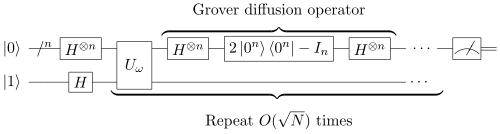
\includegraphics[scale=0.4]{Grovers_algorithm.png}

\begin{tiny}Wikipedia; Grover's algorithm\end{tiny}
\end{center}
\vspace{-0.5em}

The \textcolor{ourred}{\textsc{Sch\"{o}ning}} algorithm (walkSAT), is a classical algorithm that solves it in $O(\frac{4}{3}^{n})=O(2^{0.415n})$. We can apply Grover's search to Sch\"{o}ning's algorithm and such a quantum-ehnanced algorithm is faster than the fastest known classical algorithm[3]. But such an algorithm needs many qubits. To make everything work with fewer qubits, we reduce SAT solving to Solving PromiseBall. 

}

%----------------------------------------------------------------------------------------
%	quantum computing
%----------------------------------------------------------------------------------------

\headerbox{3. Quantum computing}{name=Image,column=1,row=0, bottomaligned=solvingSAT}{

The image below is a superconducting qubit-based quantum computer from IBM. The biggest current QC's manipulate circa 50-60 qubits. 
\begin{center}
\vspace{-1.2em}
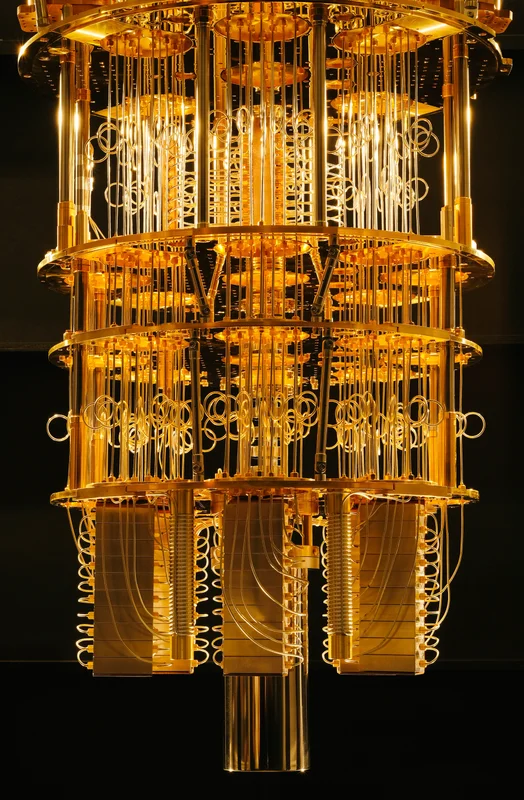
\includegraphics[scale=0.2]{quantum_computer.png}

\begin{tiny}IBM Research Flickr (2018)\end{tiny}
\end{center}

Quantum computers can be programmed by a number of programming languages. One of the most prevalent ones is \textcolor{ourred}{\textsc{Qiskit}}, which is a python library. With Qiskit I will be programming a quantum computer, where I will be optimizing code and running simulations with noise.

\begin{center}
\vspace{-1em}
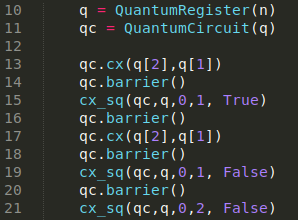
\includegraphics[scale=0.35]{Code.png}
\end{center}

}

%----------------------------------------------------------------------------------------
%	Promiseball
%----------------------------------------------------------------------------------------


\headerbox{5. PromiseBall}{name=promiseball,column=1,below=solvingSAT, bottomaligned=basics}{

The \textcolor{ourred}{\textsc{PromiseBallSAT}} (or PBS) is the central subroutine of the derandomized Sch\"{o}ning's algorithm[1][2]. Given the initial assignment $x$, let $B_{r}(x)$ denote the $r$-ball centered at $x$, i.e. the set of all bitstrings $y$ has a \textcolor{ourred}{\textsc{Hamming distance}} $\leq r$. To use PBS to solve the original kSAT problem, the space of possible assignments is covered by a number of $r$-balls.

\begin{center}
	\vspace{-0.8em}
	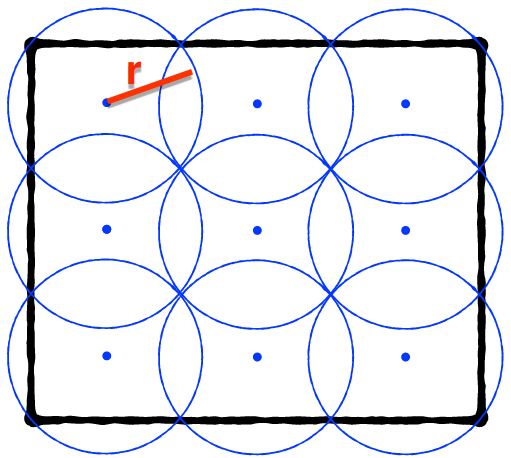
\includegraphics[scale=0.168]{PromiseBall.png}

	\begin{tiny}Vedran Dunjko (2018)\end{tiny}
	\vspace{-0.8em}
\end{center}
$Promise$-$Ball(F,r,x)$ is a deterministic recursive divide-and-conquer algorithm. It first checks conditions for (un)satisfiability, or if $x$ is a satisfying assignment. Otherwise, in the recursive step, it finds the first unsatisfied clause $C$, and recursively calls $PromiseBall(F^{[l=1]},r−1,x)$ for every literal $l\in C$. All clauses involving $l$ are removed (or truncated).

This strategy is suitable for using quantum computers that are small in size by running the classical algorithm until the recursive call becomes small enough for the limited quantum computer[4]. However, it is not clear what happens when these calls are made to a quantum device which is noisy.

	
}

%----------------------------------------------------------------------------------------
%	Quantum noise
%----------------------------------------------------------------------------------------

\headerbox{6. Quantum noise}{name=noise,column=2,below=solvingSAT}{

\textcolor{ourred}{\textsc{Quantum decoherence}}, or quantum noise, happens when qubits lose information to the environment over time. This doesn't start until the qubits are used, like measuring them or performing a computation. 

The effects of noise on real quantum computers can be studied via \textcolor{ourred}{\textsc{simulations}}, by utilizing some of the standard noise models. Quantum noise currently gets simulated by adding random gates (such as the Pauli X gate) into the circuit. I am studying the effects of noise on the performance of quantum 3-SAT solver.

}


%----------------------------------------------------------------------------------------
%	FURTHER RESEARCH
%----------------------------------------------------------------------------------------

\headerbox{7. Further research}{name=further,column=2,below=noise,bottomaligned=basics}{

\begin{enumerate}[label= {[\arabic*]}]
	\item R. A. Moser and D. Scheder, in Proceedings of the Forty-third Annual ACM Symposium on Theory of Computing, STOC '11 (ACM, New York, NY, USA, 2011) pp. 245-252.
	\item E. Dantsin, A. Goerdt, E. A. Hirsch, R. Kannan, J. Kleinberg, C. Papadimitriou, P. Raghavan, and U. Sch\"{o}ning; Theoretical Computer Science 289, 69 (2002)
	\item T. Hertli; 3-SAT Faster and Simpler - Unique-SAT Bounds for PPSZ Hold in General (2014)
	\item V. Dunjko, Y. Ge, J. I. Cirac; Computational speedup using small quantum devices (2018)
\end{enumerate}

}

%----------------------------------------------------------------------------------------

\end{poster}

\end{document}
